\documentclass[11pt,letterpaper]{article}
\usepackage[T1]{fontenc}
\usepackage{lmodern,amsmath,amssymb,amsthm,booktabs,graphicx,xcolor}
\usepackage[margin=0.88in,top=0.88in,bottom=0.88in]{geometry}
\usepackage{fancyhdr,hyperref}
\definecolor{ink}{HTML}{16374B}
\definecolor{accent}{HTML}{006B69}
\hypersetup{colorlinks=true,urlcolor=accent,linkcolor=accent,citecolor=accent,
pdftitle={Odd dyadic filters at zeros of Dirichlet L-functions}}
\pagestyle{fancy}\fancyhf{}\lhead{\small\textcolor{ink}{Odd dyadic filters}}\rhead{\small\textcolor{ink}{26 November 2026}}\cfoot{\thepage}
\setlength{\headheight}{15pt}
\setlength{\parindent}{0pt}\setlength{\parskip}{4pt plus 1pt}
\setlength{\emergencystretch}{2em}
\newtheorem{theorem}{Theorem}
\newtheorem{lemma}[theorem]{Lemma}
\newtheorem{corollary}[theorem]{Corollary}
\newcommand{\R}{\mathbb R}
\newcommand{\C}{\mathbb C}
\newcommand{\Res}{\operatorname{Res}}
\newcommand{\dd}{\,\mathrm d}
\newcommand{\art}[2]{\href{#1}{#2}}
\newcommand{\head}[1]{\par\medskip{\large\bfseries\color{ink}#1}\par\smallskip}
\begin{document}
\thispagestyle{plain}
{\small\bfseries\color{accent} RESEARCH NOTE \hfill 26 NOVEMBER 2026}
\par\vspace{0.22in}
{\huge\bfseries\color{ink} Odd dyadic filters at zeros\\[2pt] of Dirichlet \(L\)-functions\par}
\vspace{7pt}
{\large Exact minima, three active exponents, and a frequency law}\\[3pt]
Prepared for Vladimir Reshetnikov
\par\medskip
For a complex number \(z\), successive squaring produces the gains
\[
 M_n(z)=\max_{0\le j<n}|1+z^{\,2^j}|,\qquad c_n=\min_{z\in\C}M_n(z).
\]
The minimum exists since the first term tends to infinity with \(|z|\).
The ProveIt report \emph{Sharp constants for dyadic pole detection} determines
\(c_n\) for even \(n\) and for \(n=3\). It explicitly asks for the odd cases
\(n\ge5\) and their minimizers \cite{packet}. The following formula completes that family.

\begin{theorem}[Exact odd constants]\label{th:main}
Fix odd \(n\ge5\), set \(L=2^{n-1}\), \(p=\pi/3\), and put
\(y_*=(\sqrt5-1)/2\). For \(2^{-L/4}\le y\le y_*\), define
\[
 r=y^{2/L},\quad t=\frac{y(3-y^2)}{1+\sqrt{1+12y^2-4y^4}},\quad
 b=2\arcsin t,\quad A=p+\frac{b-p}{L}.
\]
There is a unique root \(y\) in this interval of the scalar equation
\begin{equation}\label{eq:scalar}
  1+r^2-2r\cos A
   =\frac32+y^2-\frac12\sqrt{1+12y^2-4y^4}.
\end{equation}
At that root, \(c_n\) is the square root of either side. The only minimizers
are \(z=r\exp(\pm i(\pi-A))\). Exactly the three exponents \(1,L/2,L\)
attain the maximum there.
\end{theorem}

For \(n=5\) the exponents are \(1,2,4,8,16\).
The terms at \(1,8,16\) attain the common maximum \(c_5=0.927585413085778\ldots\).
The other two terms are strictly smaller. A log-radius and angular change
of variables turns the comparison with every complex \(z\) into a convex
feasibility problem. This proves global optimality.

\begin{center}\small
\begin{tabular}{rccc}
\toprule
Filters & Active exponents & Optimal radius & Worst gain \(c_n\)\\\midrule
5 & \(1,8,16\) & 0.868780657 & 0.927585413\\
7 & \(1,32,64\) & 0.949460453 & 0.968754716\\
9 & \(1,128,256\) & 0.982726349 & 0.989010226\\\bottomrule
\end{tabular}
\end{center}
At a nontrivial Dirichlet \(L\)-function zero the same factors give the
change in the residue of a prime-counting transform under a two-term shift.
Theorem~\ref{th:zeta} gives the frequency with which actual zeros approach
the worst gain. It uses Dirichlet GRH and classical equidistribution.
The extremal theorem itself is elementary.

\newpage
\section{The angular sector and the scalar equation}
If \(M_n(z)<1\), every \(z^{2^j}\) is in the open left half-plane. Let
\(\alpha_j=|\arg(-z^{2^j})|\in[0,\pi/2)\), using the principal argument.
Squaring gives \(\alpha_{j+1}=\pi-2\alpha_j\). Indeed, consecutive iterates
in that half-plane require \(\alpha_j>\pi/4\) for \(j<n-1\). For odd \(n\),
with \(u=-L\log |z|\) and \(b=\alpha_{n-1}\), the recurrence gives
\begin{equation}\label{eq:angles}
  \alpha_j=p+(-1)^j\frac{2^j}{L}(b-p),\qquad
  v_j=|z|^{2^j}=e^{-2^j u/L},\qquad
  F_j=1+v_j^2-2v_j\cos\alpha_j .
\end{equation}
Conversely, for \(0<b<p\) these angles give the genuine orbit of
\(z=e^{-u/L}e^{\pm i(\pi-\alpha_0)}\). The even-indexed angles lie between
\(b\) and \(p\), the odd-indexed ones between \(p\) and
\((\pi-b)/2\). The recurrence therefore uses the same branch at every step.

The first, penultimate and last squared gains are
\begin{equation}\label{eq:pqs}
\begin{split}
 P&=1+r^2-2r\cos A,\qquad r=e^{-u/L},\qquad A=\alpha_0,\\
 Q&=1+y^2-2y\sin(b/2),\qquad y=e^{-u/2},\\
 S&=1+y^4-2y^2\cos b .
\end{split}
\end{equation}
Balancing \(Q=S\) and writing \(t=\sin(b/2)\) gives
\(4yt^2+2t=3y-y^3\). Its positive root is the expression in
Theorem~\ref{th:main}. Substitution in \(Q\) gives the right side of
\eqref{eq:scalar}. These equalities produce a candidate. The inequalities
in the next two sections certify it as the optimum.

\head{Uniqueness of the root}
For \(0<y<y_*\), \(0<t<1/2\). This follows by testing \(0\) and \(1/2\)
in the increasing quadratic, since \(1-2y+y^3>0\) on this interval.
At \(y_*\) we have \(t=1/2\), \(b=p\). Implicit differentiation gives
\[
 t'(y)=\frac{3-3y^2-4t^2}{2+8yt}>0\quad(0<y<y_*) .
\]
Here \(y_*^2<1/2\). On the interval in the theorem \(r\ge1/\sqrt2\) and
\(A\ge p(1-1/L)>\pi/4\). Thus \(P\) strictly increases with \(y\):
both the radius derivative \(2(r-\cos A)\) and the angle derivative
\(2r\sin A\) are positive. In contrast the right side of \eqref{eq:scalar}
decreases strictly up to \(y_*\). Its derivative in \(h=y^2\) is
\(1-(3-2h)/\sqrt{1+12h-4h^2}<0\) for \(0<h<(3-\sqrt5)/2\).

At the left endpoint \(y\le1/16\) and \(P\le3/2-1/\sqrt2<0.8\),
whereas \(S\ge1-2y^2>0.99\). At the right endpoint the two gains are
\(1-r+r^2\) and \(1-y_*^2+y_*^4\). The latter equals
\(1-y_*+y_*^2\) because \(1-y_*^2=y_*\). Since \(r>y_*>1/2\),
the inequality reverses. Continuity proves the asserted unique crossing.

\newpage
\section{A certificate of global optimality}
For a candidate with \(P=Q=S<1\), put \(d=1-P\), assuming \(0<d<1\).
Use the function
\[
 g_d(x)=\arccos\!\left(\frac{e^x+d e^{-x}}2\right)
 =\arccos\!\left(\sqrt d\cosh(x-\tfrac12\log d)\right)
\]
on the closed interval where its argument is at most one. It is strictly
concave. The inner function is positive and strictly convex, and
\(\arccos\) is decreasing and concave on \([0,1]\). In the sector
\eqref{eq:angles} a constraint \(F_j\le P\) is precisely
\begin{equation}\label{eq:convex}
  \alpha_j(b)\le g_d(-2^j u/L),
\end{equation}
with the argument in the domain of \(g_d\). This angle function also
appears in the even-case proof of \cite{packet}.

\begin{lemma}[Three supporting directions]\label{lem:certificate}
Suppose the scalar root satisfies \(0<d<1\) and \(P>F_1\).
If the gradients of \(P,Q,S\) in \((u,b)\) have a strictly positive
linear combination equal to zero and span \(\R^2\), then the conclusions
about \(c_n\), the minimizers and the active exponents in
Theorem~\ref{th:main} hold.
\end{lemma}

\begin{proof}
On each parity of \(j\), the angle in \eqref{eq:angles} is affine in
the exponent \(k=2^j\), and \(g_d(-ku/L)\) is strictly concave in \(k\)
since \(r<1\). The outer exponents of the even-indexed set are \(1,L\);
those of the odd-indexed set are \(2,L/2\). The endpoint constraints follow
from the hypotheses. The interval domain is convex. Interpolation proves
strict inequality for all interior exponents. Both constructed points
therefore attain \(\sqrt P\).

Consider any \(z'\) with \(M_n(z')\le\sqrt P<1\). Its \((u',b')\)
satisfies all three active inequalities. At the constructed point the
three convex functions \(\alpha_j(b)-g_d(-2^ju/L)\) vanish. They are
differentiable there since all three contact angles are strictly positive.
Their tangent inequalities give a nonpositive inner product between
each gradient and the displacement \((u'-u,b'-b)\). At contact, the gradient
of \(F_j\) equals the respective gradient of the convex function times
\(2v_j\sin\alpha_j>0\). This follows by differentiating
\(1+v_j^2-2v_j\cos(g_d(\log v_j))=P\).
The positive combination in the hypothesis forces all three inner
products to vanish. Spanning then forces the displacement to vanish.
The only two complex points with those coordinates are the stated conjugates.
\end{proof}

For later checks the three gradients, in the same order, are
\begin{equation}\label{eq:grad}
 \left(-\frac{2r(r-\cos A)}{L},\frac{2r\sin A}{L}\right),\quad
 \bigl(y(t-y),-y\cos(b/2)\bigr),\quad
 \bigl(2y^2(\cos b-y^2),2y^2\sin b\bigr).
\end{equation}
Thus a gap to the remaining exponents and three ordinary plane vector
directions suffice to rule out every competitor, including points with
radius greater than one.

\newpage
\section{Verification for all odd indices}
\head{The uniform range \(L\ge2^{20}\)}
First locate the scalar root in \(\tfrac12\log L\le u\le2\log L\).
Throughout this interval \(r\ge .999\), \(y\le1/32\). Writing
\(t=y f(y^2)\), the formula for \(t\) gives
\(1.49\le f\le1.5\) by bounding its numerator and denominator at
\(0\) and \(1/1024\). Hence \(0<b<0.1\).
As \(|A-p|\le p/L\), the 1-Lipschitz bound on cosine gives
\[
 .99u/L\le r(1-r)\le 1-P\le (u+2p)/L,\qquad
 y^2\le 1-S\le 2y^2 .
\]
We used \(1-r\ge r u/L\) and \(\cos A\ge1/2\). At
\(u=\tfrac12\log L\) one has \(\sqrt L>\tfrac12\log L+2p\), so
\(P>S\). At \(u=2\log L\), \(1.98L\log L>2\) gives \(P<S\).
This interval has \(r>1/\sqrt2\) and \(y<y_*\), so its crossing
is the root already proved unique. Also \(0<P<1\) there.

For \(F_1\), the angle at exponent \(2\) differs from \(p\) by at most
\(2p/L\). Replacing the two angles of \(P,F_1\) by \(p\) gives
\[
 P-F_1\ \ge\ r(1-r)(r^2+r-1)-\frac{6p}{L}
           \ \ge\ \frac{.99u-2\pi}{L}>0.
\]
For the second inequality, \(r^2(r^2+r-1)>.99\) at \(r\ge.999\);
for the last, \(u\ge10\log 2\). In \eqref{eq:grad} the first vector points
left and up with slope between \(-3\) and \(-1\)
(use \(p-p/L\le A\le p\), \(r\ge.999\)).
The second points right and down with slope
\(-\cos(b/2)/(y(f-1))<-60\). The third points right and up.
The negative of the first is strictly between the other two directions.
Lemma~\ref{lem:certificate} applies.

\head{The eight smaller odd indices}
The following finite certificate uses only integer arithmetic and square
roots. Its fixed denominator for \(y\) is \(2^{24}\). Each root lies in
\([k,k+1]/2^{24}\); the listed margin is a lower bound for
\(\min_{j\notin\{0,n-2,n-1\}}(P-F_j)\) at the root.
\begin{center}\small
\begin{tabular}{rrc@{\hspace{0.55in}}rrc}
\toprule
\(n\)&\(k\)& Margin &\(n\)&\(k\)& Margin\\\midrule
5&5445039&\(2^{-12}\)&13&541603&\(2^{-12}\)\\
7&3191391&\(2^{-10}\)&15&290764&\(2^{-13}\)\\
9&1803402&\(2^{-10}\)&17&154678&\(2^{-14}\)\\
11&996494&\(2^{-10}\)&19&81717&\(2^{-16}\)\\\bottomrule
\end{tabular}
\end{center}
The next page specifies every test that gives these bounds. Across all
eight rows the endpoint sign margins are at least \(2^{-34}\), and all
three normalized determinant margins are at least \(1/4\).
\newpage
\head{How to reproduce the finite proof}
Use \(d_j=1-F_j\), \(C_j=\cos\alpha_j\) and \(v_j=|z|^{2^j}\).
On each printed interval form \(w=2t\) and the pairs
\[
 (v_{n-1},C_{n-1})=(y^2,1-w^2/2),\quad
 (v_{n-2},C_{n-2})=(y,w/2),\quad
 (v_{j-1},C_{j-1})=\left(\sqrt{v_j},\sqrt{(1-C_j)/2}\right).
\]
The last rule is applied backwards from \(j=n-2\) to \(j=1\).
It follows from \(\alpha_{j-1}=(\pi-\alpha_j)/2\).
In \((\log v_{n-1},b)\) coordinates, the gradient of \(d_j\), divided by
\(2(2^j/L)v_j>0\), is
\[
 g_j=\bigl(C_j-v_j,\,-(-1)^j\sqrt{1-C_j^2}\bigr).
\]
Negating all vectors, changing coordinates by a reflection, and scaling
individual vectors by positive factors preserve the positive-span property.

At the left endpoint verify \(d_0-d_{n-1}>0\) and at the right endpoint
verify \(d_{n-1}-d_0>0\). Over the whole interval verify
\(2y<1,\ 2r^2>1,\ 0<C_j<1,\ 0<d_{n-1}<1\). Also verify
\(d_j-d_{n-1}>0\) at every inactive index.
For the cyclic list \(g_0,g_{n-2},g_{n-1}\), all three consecutive
determinants, including the wraparound pair, are negative.
Indeed \(\det(v,w)u+\det(w,u)v+\det(u,v)w=0\) for any three plane vectors.
The strict signs provide the positive combination and spanning required by
Lemma~\ref{lem:certificate}. This completes the proof of Theorem~\ref{th:main}.

The enclosed \texttt{code/verify\_finite.py} performs exactly these operations
with integer endpoints on a grid of spacing \(2^{-256}\). It rounds each
interval outwards and encloses square roots using integer square root.
The opposite signs certify existence; the entire interval certifies the
strict inequalities at the root. The printed interval endpoints also
allow this short computation to be repeated independently.
The half-angle recursion shows that \eqref{eq:scalar} can be evaluated
entirely with radicals starting from \(y\). In particular the answer is an
algebraic number: the unique admissible root is an isolated point of a set
defined by polynomial equations and inequalities over the rationals (introduce
a nonnegative variable for each square root).

\head{Keeping only the three active shifts}
There is a distinction between a contact at a minimizer and an observation
which can be deleted. For odd \(n\ge5\) one has
\[
 \min_{z\in\C}\max\{|1+z|,|1+z^{L/2}|,|1+z^L|\}=c_2=\sqrt{3-\sqrt5}.
\]
The last two terms alone give the lower bound by the classical two-filter
problem \cite{contest}. To attain it let \(q=(\sqrt5-1)/2\) and choose
\(z=-q^{2/L}\exp(4\pi i/(3L))\). Then \(z^{L/2}=q e^{2\pi i/3}\),
a two-filter minimizer. The first term is bounded by
\(1-q^{2/L}+4\pi/(3L)<1/2\), using \(L\ge16\), \(q>1/2\).
The full family obeys \(c_n\ge c_3=0.882003\ldots>c_2\) by
\cite{packet}. Thus the omitted observations impose a real restriction
even though they are slack at the two global minimizers.

\newpage
\section{The parity correction}
Let \(W(x)\) denote the positive root of \(W e^W=x\). The even formula in
\cite{packet} gives \(2L(1-c_n)=W(L)+O(W(L)^2/L)\) along even \(n\).
The odd case has a persistent offset after the same normalization.

\begin{theorem}\label{th:asymptotic}
Along odd \(n\to\infty\), put \(a_0=\pi/\sqrt3\), \(Y=W(2e^{a_0}L)\).
Then
\begin{equation}\label{eq:expansion}
 2L(1-c_n)
 =Y-\frac{3\sqrt3\,Y}{1+Y}\sqrt{\frac{Y}{2L}}
       +O\!\left(\frac{Y^2}{L}\right).
\end{equation}
In particular the odd subsequence of \(2L(1-c_n)-W(L)\) tends to
\(\log 2+\pi/\sqrt3\), while the even subsequence tends to zero.
\end{theorem}

\begin{proof}
Write \(\lambda=L(1-c_n^2)\). The uniform bracket gives
\(u\asymp\log L\), \(y=o(1)\). The quadratic for \(t\) gives
\(t=3y/2+O(y^3)\), so \(b=3y+O(y^3)\).
Expand \(r=e^{-u/L}\) and \(\cos A\) in \(P\); expand \(\cos b\) in \(S\).
The contacts give
\[
 \lambda=u+a_0-3\sqrt3\,y+O(u^2/L+y^3),\qquad
 \lambda=2Ly^2\{1+O(y^2)\}.
\]
In the first equality the angular contribution is
\(2\sin(p)(p-b)=a_0-\sqrt3 b\). It follows that
\(\lambda\asymp\log L\),
\(y=\sqrt{\lambda/(2L)}\{1+O(\lambda/L)\}\), and
\(u=-2\log y=\log(2L/\lambda)+O(\lambda/L)\). Hence
\[
 \lambda+\log\lambda
 =\log(2L)+a_0-3\sqrt3\sqrt{\lambda/(2L)}
     +O(\lambda^2/L).
\]
The left side equals \(\log(2L)+a_0\) at \(\lambda=Y\), and its derivative
is at least one. First \(\lambda-Y=O(\sqrt{Y/L})\), since \(Y\asymp\log L\).
Taylor expansion at \(Y\) then gives
\((1+1/Y)(\lambda-Y)=-3\sqrt3\sqrt{Y/(2L)}+O(Y^2/L)\).
The identity \(2L(1-c_n)=\lambda+O(\lambda^2/L)\) proves the expansion.
Finally \(W(CL)-W(L)\to\log C\) for fixed \(C>0\), by applying the mean
value theorem to \(x+\log x\).
\end{proof}

\begin{center}
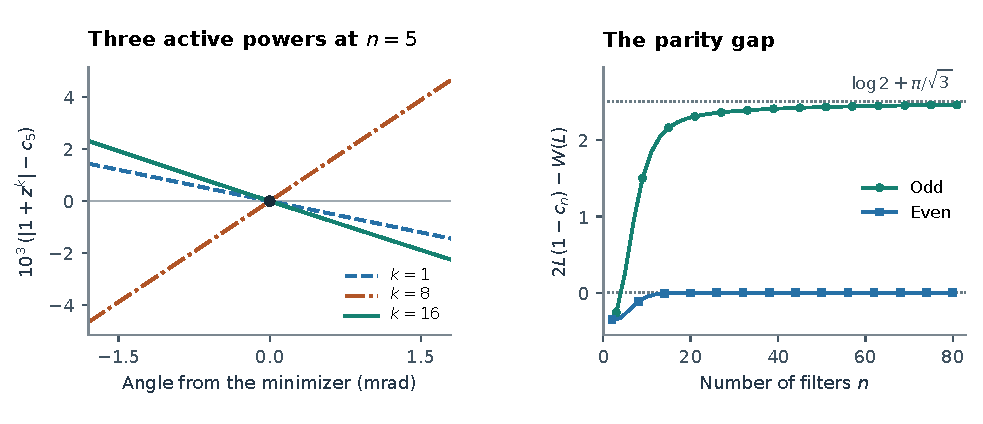
\includegraphics[width=.94\linewidth]{figures/dyadic_contacts.pdf}
\end{center}
{\small\textbf{Figure 1.} Numerical illustrations. The three active gains meet
on the optimal circle for \(n=5\) (left). The parity correction approaches
two different limits (right). The \(\mathrm{CSV}\) and generating program
in the archive reproduce the figure.}

\newpage
\section{Sharpness at actual Dirichlet zeros}
Fix a Dirichlet character \(\chi\) of positive modulus and write
\(D(s)=L(s,\chi)\). The character modulo one gives \(D=\zeta\).
Define \(\psi_\chi(x)=\sum_{m\le x}\chi(m)\Lambda(m)\),
\(E(t)=e^{-t}\psi_\chi(e^t)\), and fix a delay \(h>0\) and weight \(a>0\). Write
\[
  E_j(t)=E(t)+a^{2^j}E(t+2^jh),\qquad
  \mathcal F[U](s)=\int_0^\infty U(t)e^{(1-s)t}\dd t .
\]
For \(\Re s>1\), direct integration of the absolutely convergent
Dirichlet series gives \(F(s)=\mathcal F[E](s)=-D'(s)/(sD(s))\).
At any zero \(\rho\) in the open critical strip, of multiplicity \(m_\rho\), \(F\) has
a simple pole of nonzero residue \(-m_\rho/\rho\). A change of variable gives
\[
 \mathcal F[E_j](s)=(1+z(s)^k)F(s)
    -z(s)^k\int_0^{kh} E(t)e^{(1-s)t}\dd t,\quad
 k=2^j,\quad z(s)=a e^{h(s-1)} .
\]
The finite integral is entire, so this identity continues meromorphically.
Define the normalized gain
\(G_n(\rho)=\max_j|\Res_\rho\mathcal F[E_j]|/|\Res_\rho F|\).
Then \(G_n(\rho)=M_n(z(\rho))\) exactly.

\begin{theorem}[Critical-line frequency law]\label{th:zeta}
Let \(r,b,A,y\) be the solution in Theorem~\ref{th:main}. For every fixed
\(h>0\), choose \(a=r e^{h/2}\). Over the open-strip zeros of \(D\),
\(\rho=\tfrac12+i\gamma,\ \gamma>0\), counted with multiplicity,
\(\inf_\rho G_n(\rho)=c_n\). For each sufficiently small fixed
\(\epsilon>0\), the proportion with \(G_n(\rho)\le c_n+\epsilon\)
among \(0<\gamma\le T\) has a limit \(D_n(\epsilon)\) as \(T\to\infty\).
Moreover
\begin{equation}\label{eq:frequency}
 D_n(\epsilon)=K_n\epsilon+O_n(\epsilon^2),\qquad
 K_n=\frac{c_n}{\pi}\left[
 \frac{1}{\max(r\sin A,Ly^2\sin b)}
 +\frac{2}{Ly\cos(b/2)}\right].
\end{equation}
In particular \(K_n\to2/(\pi\sqrt3)\) along odd \(n\). The order of limits
is first \(T\to\infty\), then \(\epsilon\downarrow0\), then odd \(n\to\infty\).
\end{theorem}

\begin{proof}
Dirichlet GRH fixes the radius at \(r\) for every open-strip zero. For a
primitive \(\chi\), the degree-one Landau formula at each fixed \(x=e^{kh}>1\)
gives \(\sum_{0<\gamma\le T}x^\rho=O_{k,h,\chi}(T)\).
The zero count is asymptotic to \(T\log T/(2\pi)\)
\cite[eq.~(2.1) and Lemma 2.1]{fzl}. Since \(x^\rho=e^{kh/2}e^{ikh\gamma}\),
Weyl's criterion gives uniform distribution of \(h\gamma\bmod 2\pi\).
For zeta this is the classical argument in \cite{fz}. For imprimitive
\(\chi\), the extra Euler factors \(1-\chi^*(\ell)\ell^{-s}\) attached to
its inducing primitive character \(\chi^*\) have no zeros in \(\Re s>0\);
the open-strip zeros and their multiplicities agree. Hence the limiting
proportion is the normalized angular length of the sublevel set. Its boundary is finite, since it is contained
in a finite union of level sets of nonconstant cosines. Continuity and the
two minimizing angles give the stated infimum.

Near either minimizer use \(b\) as a coordinate on the fixed circle;
\(|\dd b/\dd\theta|=L\). The inactive terms have a strict gap. The squared
terms \(P,S\) have positive \(b\)-derivatives, and \(Q\) has a negative one,
given in \eqref{eq:grad}. In angular distance the two outward slopes of the
gain are \(s_+=\max(r\sin A,Ly^2\sin b)/c_n\) and
\(s_-=(L/2)y\cos(b/2)/c_n\), up to exchange. Thus the angular sublevel
length near each minimum is \(\epsilon(1/s_++1/s_-)+O_n(\epsilon^2)\).
Compactness excludes any other arc for sufficiently small \(\epsilon\).
Two minima and division by \(2\pi\) give \eqref{eq:frequency}. Finally
\(r\to1\), \(A\to p\), \(Ly^2\sin b=O(Ly^3)\to0\), and \(Ly\to\infty\)
by Theorem~\ref{th:asymptotic} and its proof.
\end{proof}

For exact equality at a \emph{prescribed} positive ordinate \(\gamma\),
choose \(h=(\pi-A)/\gamma\) and \(a=r e^{h/2}\). Then
\(z(\tfrac12+i\gamma)=r e^{i(\pi-A)}\) exactly. At a fixed delay, the
frequency theorem instead allows one to keep the same observations at every zero.

\newpage
\section{Relation to the supplied sources}
The readable Lean project at commit \texttt{72fead10} states the zeta and
Dirichlet theorems using Mathlib's functions. Its Dirichlet result applies
to characters of every positive modulus, including imprimitive characters,
in the open critical strip. In the right-half-plane nonvanishing version,
the principal-character pole has its own exception. The project's reading
guide identifies a chain of lattice comparisons leading to a one-sided
bound for a smoothed prime remainder. The final analytic step interprets
zeros through the poles of a transform \cite{lean}. Andrew Sutherland
records independent builds of the shortened development and its three
standard Lean axioms \cite{sutherland}. We inspected the sources and used the published build record.

The supplied Wikipedia article presents the critical-line theorem together
with the explicit formula connecting zeros to oscillations of prime counts
\cite{wiki}. The logarithmic derivative gives a prime-counting transform
whose residues remain nonzero even at a multiple zero. For general \(a,h\),
the infimum over the positive-ordinate zeros of any fixed \(D\) is
\(\min_\theta M_n(ae^{-h/2}e^{i\theta})\), by the same equidistribution
argument. Compactness and uniqueness in Theorem~\ref{th:main} give equality
to \(c_n\) precisely when \(a e^{-h/2}=r\). For the signed difference of
multiplicities in the Lean project's prime remainder, additional arithmetic
cancellation can occur before a filter is applied.

The ProveIt directory indexes 61 placed packets and describes their local
verification status. We compared that catalogue and the adjacent incoming
packets. The closest predecessor is the dyadic pole-detection packet at
commit \texttt{b9a7c196}. Its even family, three-filter quartic, transform
identity, and discussion of the two-filter contest problem give the starting
point \cite{packet,contest}. The results claimed here are the odd family
\(n\ge5\), its three contacts and minimizers, the parity correction and the
small-tolerance law for Dirichlet zero residues. Searches for the dyadic
extremal problem and its polynomial variants identified the earlier
two-filter problem. Historical priority beyond the material located remains
unverified. The new theorem has a mathematical proof with an exact finite
certificate. A Lean formalization of this extension remains open.

\head{Further research}
A natural next problem is to obtain a \(T\)-dependent error term in
\eqref{eq:frequency} when the tolerance decreases with the height. This
requires controlling the discrepancy of \(h\gamma\) in shrinking arcs.
A second question is whether deleting any single exponent from a long
dyadic family permits an exact classification of the resulting minima.

{\small
\begin{thebibliography}{9}\setlength{\itemsep}{1pt}
\bibitem{packet} V. Reshetnikov, \art{https://github.com/VladimirReshetnikov/ProveIt/tree/b9a7c196e4aed3d93d4f222efef677a50efe912b/Analysis/GeneralizedRiemannHypothesis}{\emph{ProveIt}, Generalized Riemann Hypothesis collection}.
\art{https://github.com/VladimirReshetnikov/ProveIt/blob/b9a7c196e4aed3d93d4f222efef677a50efe912b/Analysis/GeneralizedRiemannHypothesis/docs/incoming/dyadic_pole_detection_2026-11-26.zip}{\emph{Sharp constants for dyadic pole detection}}, 26 Nov.\ 2026, especially the even theorem, the three-filter theorem, and the final questions.
\bibitem{lean} L. Sernau and collaborators, \art{https://github.com/lsernau/grh-lean/tree/72fead102f663d5c7a407964a13dc0cf9d977207}{\emph{GRH for Dirichlet \(L\)-functions, in Lean 4}}.
\art{https://github.com/lsernau/grh-lean/blob/72fead102f663d5c7a407964a13dc0cf9d977207/grh/src/Statements.lean}{Statements},
\art{https://github.com/lsernau/grh-lean/blob/72fead102f663d5c7a407964a13dc0cf9d977207/grh/GUIDE.md}{reading guide}, and
\art{https://github.com/lsernau/grh-lean/blob/72fead102f663d5c7a407964a13dc0cf9d977207/grh/src/New/Reduction/OneSidedBound.lean}{one-sided bound}.
\bibitem{sutherland} A. Sutherland, \art{https://math.mit.edu/~drew/shortgrh/}{\emph{Verification files for the shorter Lean proof of RH and GRH}}, Nov.\ 2026.
\bibitem{wiki} Wikipedia contributors, \art{https://en.wikipedia.org/wiki/Riemann_hypothesis}{\emph{Riemann hypothesis}}, consulted 26 Nov.\ 2026.
\bibitem{contest} G. Sz\'asz et al., eds., \art{https://real-eod.mtak.hu/14558/1/AkademiaiKiado_007070.pdf}{\emph{Contests in Higher Mathematics, Hungary 1949--1961}}, Akad\'emiai Kiad\'o, 1968, \S3.3, problem 2.
\bibitem{fz} K. Ford and A. Zaharescu, \art{https://arxiv.org/abs/math/0405459}{On the distribution of imaginary parts of zeros of the Riemann zeta function}, \emph{J. reine angew. Math.} \textbf{579} (2005), 145--158, introduction and (1.1)--(1.2).
\bibitem{fzl} K. Ford and A. Zaharescu, \art{https://doi.org/10.1112/S0010437X14007659}{Unnormalized differences between zeros of \(L\)-functions}, \emph{Compos. Math.} \textbf{151} (2015), 230--252, \S2.
\end{thebibliography}}
\end{document}
